\documentclass[tikz]{standalone}
\usepackage{wasysym}
\usepackage{SIunits}
\usepackage{pgfplots}
\pgfplotsset{compat=1.5}
\usetikzlibrary{plotmarks,arrows}
\tikzset{>=latex}

\definecolor{tissueColour}{RGB}{255,255,255}
\definecolor{lesionColour}{RGB}{200,200,200}
\definecolor{fatColour}{RGB}{100,100,100}
\definecolor{boneColour}{RGB}{0,0,0}
\begin{document}
	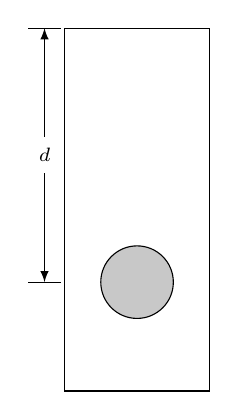
\begin{tikzpicture}[x=0.038\textwidth, y=0.038\textwidth]
		% the main domain area
		\draw[fill=tissueColour] (0, 0) rectangle(4, 10);

		% the lesion
		\draw[fill=lesionColour] (2, 3) circle(1);

		% lesion depth
		\draw (-1, 10) -- (-0.1, 10);
		\draw (-1, 3) -- (-0.1, 3);
		\draw (-0.55, 6.5) node{\scriptsize $d$};
		\draw[<-] (-0.551, 10) -- (-0.551, 7);
		\draw[->] (-0.551, 6) -- (-0.551, 3);
	\end{tikzpicture}
\end{document}